%======================================================================
\chapter{The Proposed Method}
%======================================================================
The study of the previous methods revealed that fine details and textures convey valuable information for assessing multiple distortions. Therefore, we consider such features and propose a FR and a NR method for assessing the quality of multiply-distorted images.

For preserving the speed of execution, it is desired that expressing the texture does not add a significant computational load to the algorithm. On the one hand, gradient directions are implicitly computed for calculating the gradient magnitude and on the other hand, gradient directions are more sensitive to fine details than gradient magnitude. So, we describe the macro-structures with gradient magnitude and the micro-structures with gradient direction.

By combining the similarity of gradient magnitude with the similarity of gradient direction in a FR method, we could increase the accuracy for multiply distorted images in an acceptable time.

To employ gradient direction in NR manner, the histogram of LBP values were used to construct the features vector. The relation between micro and macro structures is an effective feature of the current methods. In the proposed method, this relation is considered by weighting the histograms with gradient magnitude. Experiments show that the resultant generality of the method justifies the added features. The proposed FR and NR algorithms are presented in subsequent sections.
% -------------------------------------------
\section{Gradient Direction Similarity}
% -------------------------------------------
Gradient directions are a good representative for human detection~\cite{Dalal2005} and texture~\cite{Wu2015}. Fig.~\ref{fig:sample_dir_dir} shows the gradient directions for a sample image.
\begin{figure}
     \centering
     \begin{subfigure}[b]{0.3\textwidth}
         \centering
         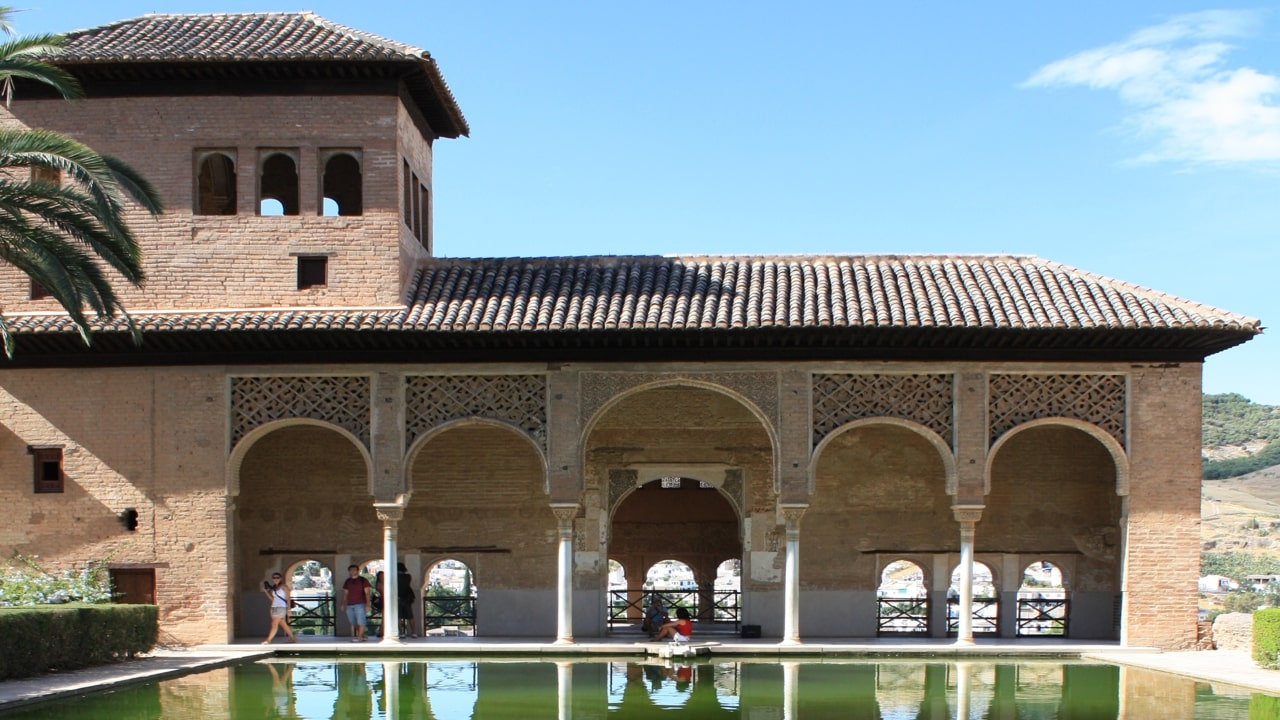
\includegraphics[width=\textwidth]{./figs/org009}
         \caption{}
         \label{fig:sample_dir}
     \end{subfigure}
     \hfill
     \begin{subfigure}[b]{0.3\textwidth}
         \centering
         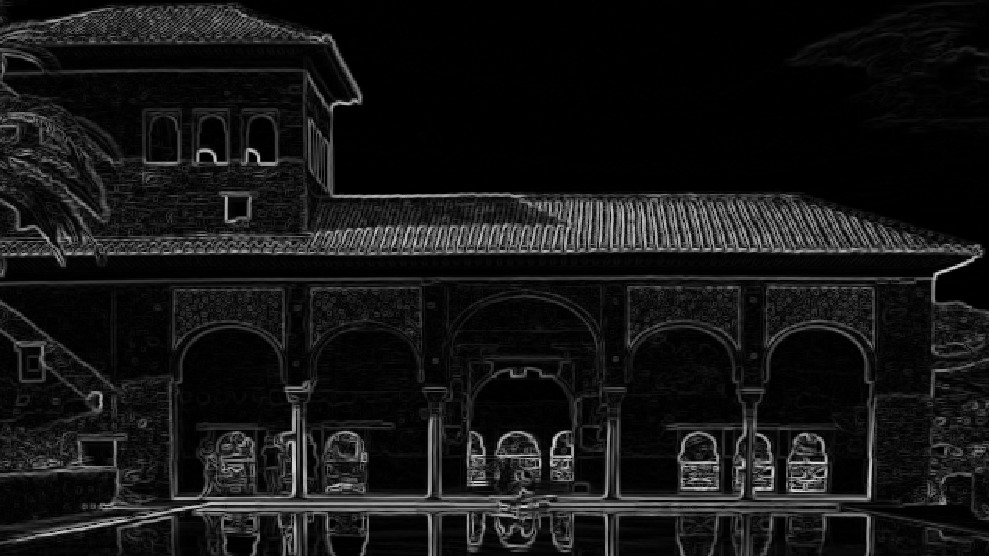
\includegraphics[width=\textwidth]{./figs/mg_map_ref}
         \caption{}
         \label{fig:sample_dir_mag}
     \end{subfigure}
     \hfill
     \begin{subfigure}[b]{0.3\textwidth}
         \centering
         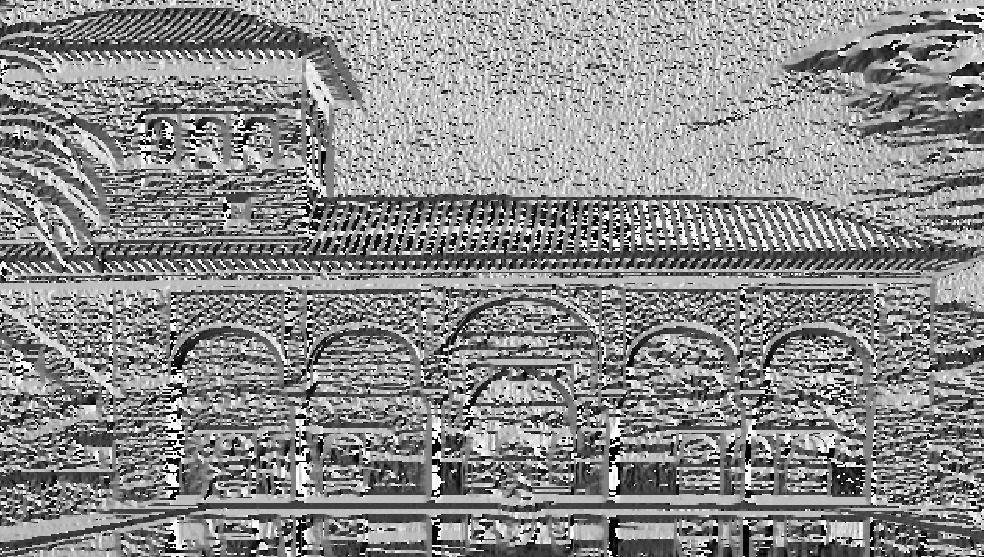
\includegraphics[width= \textwidth]{./figs/dir_ref}
         \caption{}
         \label{fig:sample_dir_dir}
     \end{subfigure}
     \caption{Magnitude and direction of gradient vectors for an image in (b) and (c), respectively.}
        \label{fig:sample_dir}
\end{figure}
It is seen that direction is more sensitive to fine details. In~\cite{Xue2014} gradient magnitude similarity is used for assessing single distortions. This similarity is defined in~\ref{eq:gms}. Gradient magnitude is attributed to extract the coarse structures of an image~\cite{xue2014blind} and we incorporate gradient directions for studying the effect micro-structures on the perceived quality of multiply-distorted images. If the direction of a gradient vector is defined as~\ref{eq:gd}, the gradient direction similarity map of the images, $r$ and $d$, is called $GDS$ and obtained as:
\begin{equation}
    GDS(r, d)_{(x, y)}=\frac{2\times GD_r(x, y)\times GD_d(x, y)+c}{GD_r(x, y)^2+GD_d(x, y)^2 +c}
    \label{eq:gd_similarity}
\end{equation}
Where, $GD_r$ and $GD_d$ are the gradient direction maps of $r$ and $d$, and $c$ is a constant for avoiding the instability of the fraction. It is seen in Fig.~\ref{fig:dir_dsts} that gradient direction is sensitive to image artifacts.
\begin{figure}
     \centering
     \begin{subfigure}[b]{0.24\textwidth}
         \centering
         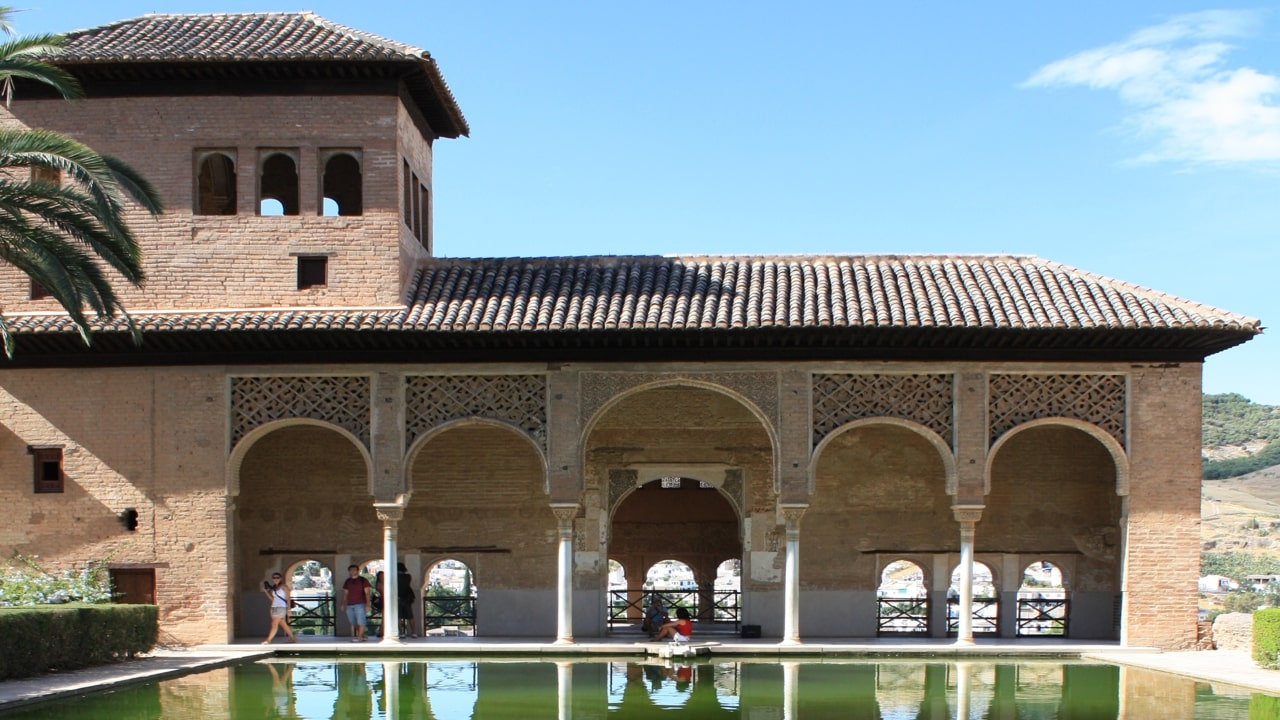
\includegraphics[width=\textwidth]{./figs/org009}
         %\caption{}
         %\label{}
     \end{subfigure}
     \hfill
     \begin{subfigure}[b]{0.24\textwidth}
         \centering
         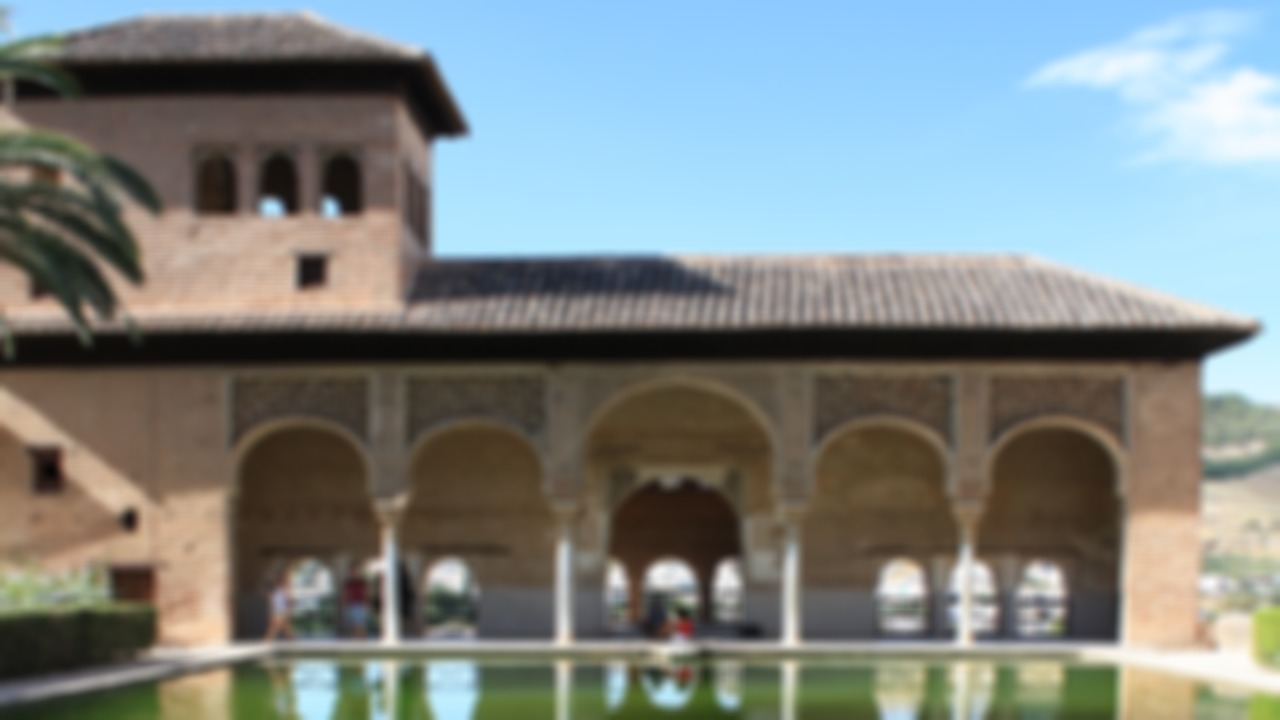
\includegraphics[width=\textwidth]{./figs/blur3}
         %\caption{}
         %\label{fig:sample_dir_mag}
     \end{subfigure}
     \hfill
     \begin{subfigure}[b]{0.24\textwidth}
         \centering
         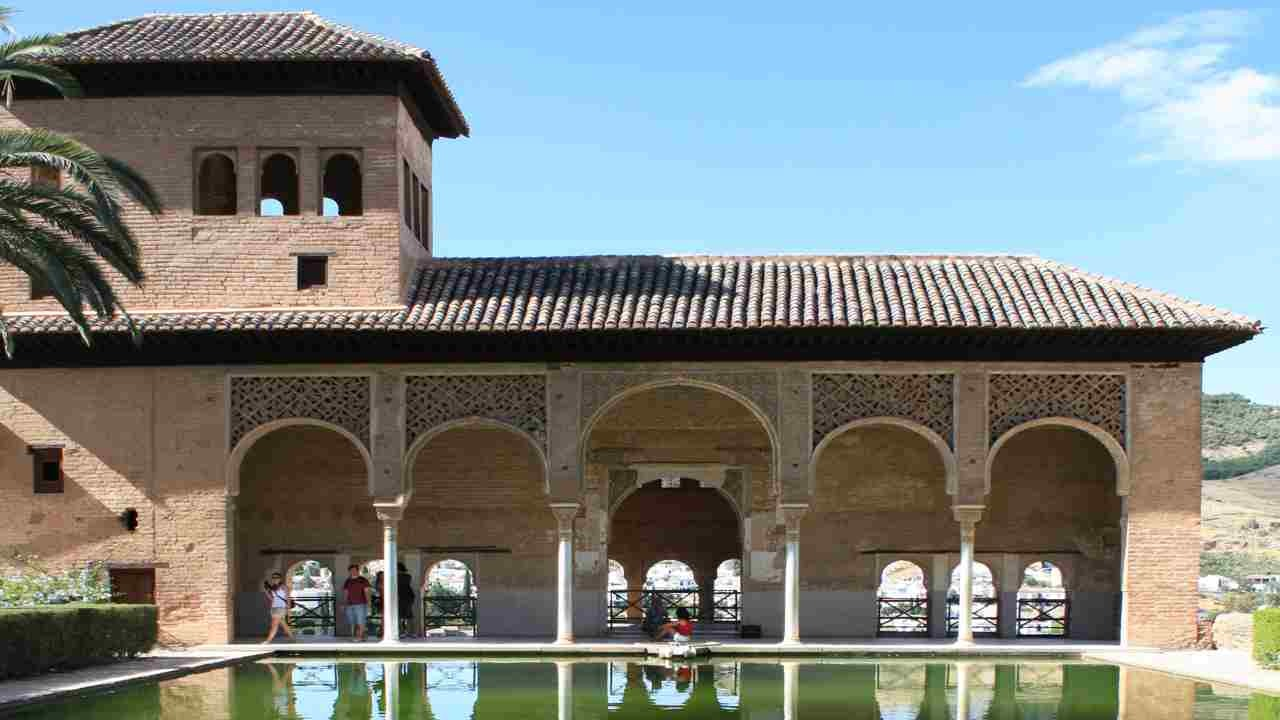
\includegraphics[width= \textwidth]{./figs/jpeg3}
         %\caption{}
         %\label{fig:sample_dir_dir}
     \end{subfigure}
     \hfill
     \begin{subfigure}[b]{0.24\textwidth}
         \centering
         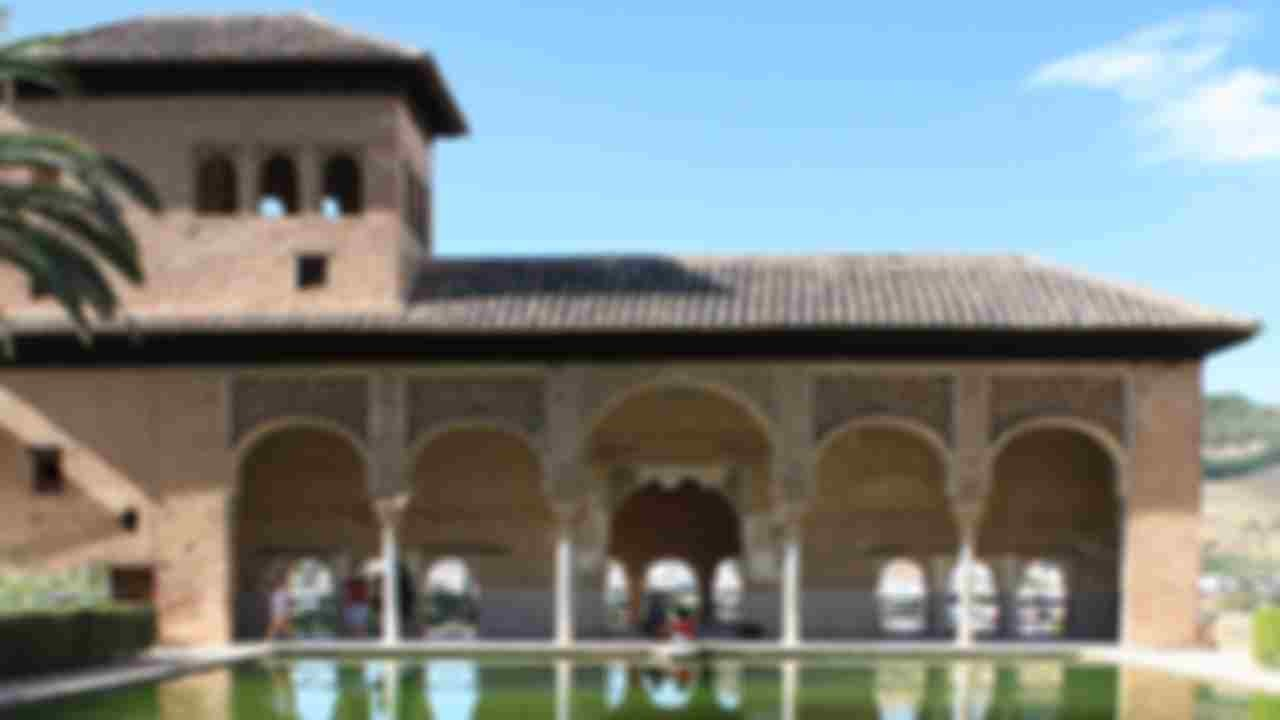
\includegraphics[width= \textwidth]{./figs/blur3_jpeg3}
         %\caption{}
         %\label{fig:sample_dir_dir}
     \end{subfigure}\\
     \begin{subfigure}[b]{0.24\textwidth}
         \centering
         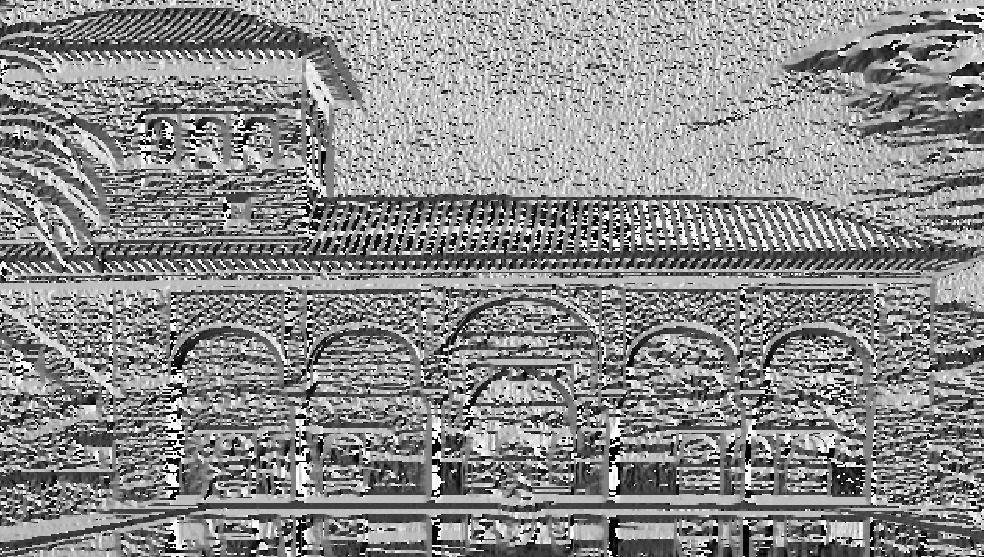
\includegraphics[width=\textwidth]{./figs/dir_ref}
         \caption{Reference}
         %\label{fig:sample_dir}
     \end{subfigure}
     \hfill
     \begin{subfigure}[b]{0.24\textwidth}
         \centering
         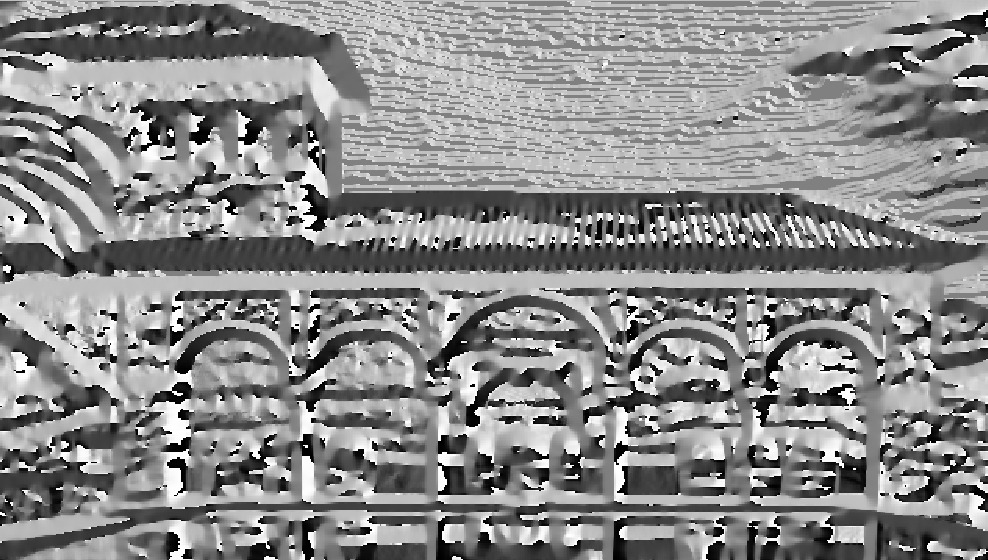
\includegraphics[width=\textwidth]{./figs/dir_blur3}
         \caption{Blur}
         %\label{fig:sample_dir_mag}
     \end{subfigure}
     \hfill
     \begin{subfigure}[b]{0.24\textwidth}
         \centering
         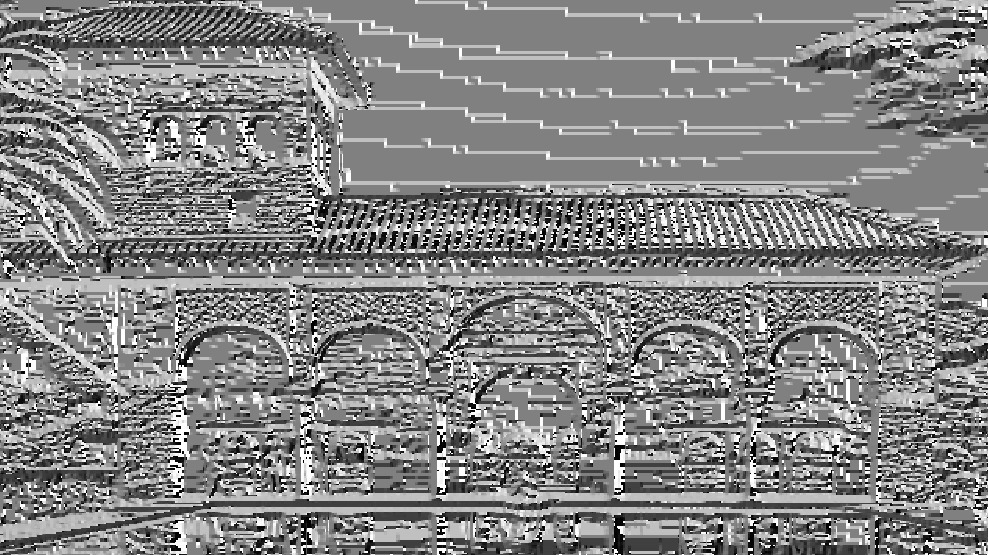
\includegraphics[width= \textwidth]{./figs/dir_jpeg3}
         \caption{Jpeg}
         %\label{fig:sample_dir_dir}
     \end{subfigure}
     \hfill
     \begin{subfigure}[b]{0.24\textwidth}
         \centering
         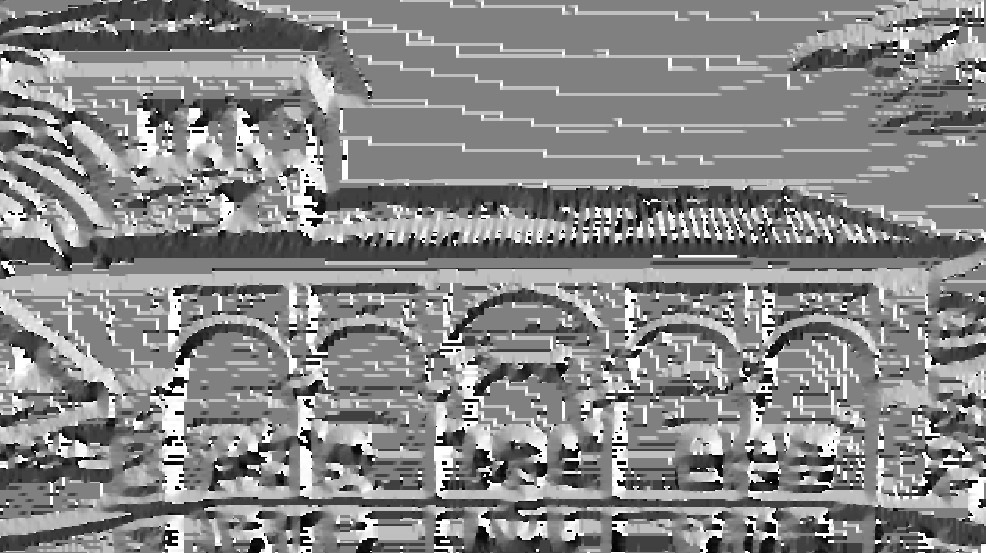
\includegraphics[width= \textwidth]{./figs/dir_blur3_jpeg_3}
         \caption{Blur \& Jpeg}
        % \label{fig:sample_dir_dir}
     \end{subfigure}
     \caption{Sensitivity of gradient direction to various artifacts}
        \label{fig:dir_dsts}
\end{figure}
With the point-wise multiplication of $GDS$ and $GMS$, the gradient similarity map is obtained, which we address it as $GS$:
\begin{equation}
    GS(r, d)_{(x, y)} = GMS(r, d)_{(x, y)}\times GDS(r, d)_{(x, y)}
    \label{eq:gradien t_similarity}
\end{equation}
For collapsing the values of $GS$ to a single score, a weighted average of its values is computed. The weight of each pixel is equal to maximum of gradient magnitude from either the reference or the distorted image:
\begin{equation}
    W(x, y) = max\left\{ GM_r(x, y), GM_d(x, y)\right\}
    \label{eq:weight_gs}
\end{equation}
So the quality score is defined as below:
\begin{equation}
    Q = \frac{\sum_x\sum_y W(x, y)\times GS(x, y)}{\sum_x\sum_y W(x, y)} \in [0, 1]
    \label{eq:frscore}
\end{equation}
A more accurate prediction is achieved with computing the direction similarity and weighting with gradient magnitude. Instead of considering $\theta$ and $-\theta$ as two different directions, we can use the absolute value of~\ref{eq:gd} as the `gradient direction':
\begin{equation}
    GD_I(x, y) = \left|tan^{-1}\left(\frac{g_v}{g_h}\right)\right|
    \label{eq:absdir}
\end{equation}
\begin{figure}
     \centering
     \begin{subfigure}[b]{0.49\textwidth}
         \centering
         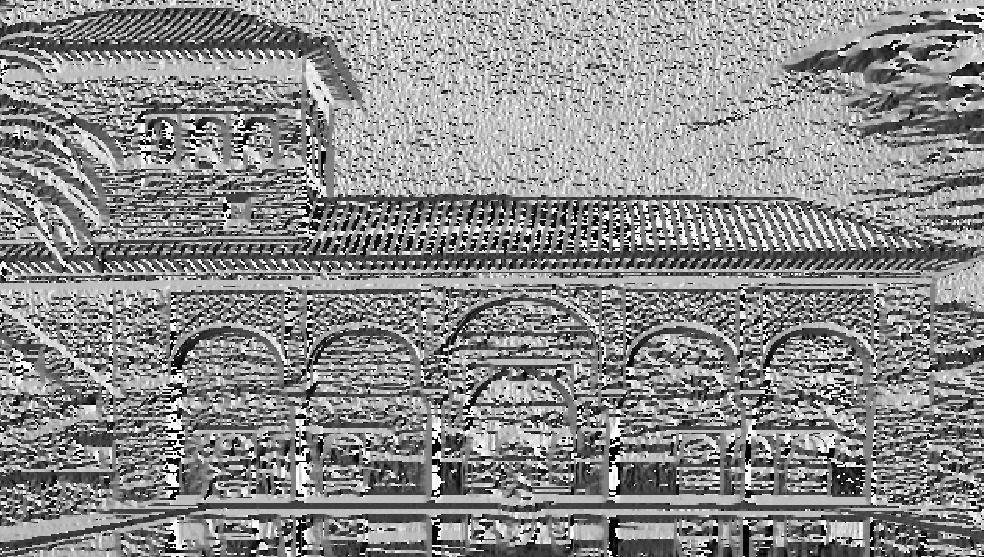
\includegraphics[width=\textwidth]{./figs/dir_ref}
         \caption{tangent inverse}
         \label{fig:tantan}
     \end{subfigure}
     \hfill
     \begin{subfigure}[b]{0.49\textwidth}
         \centering
         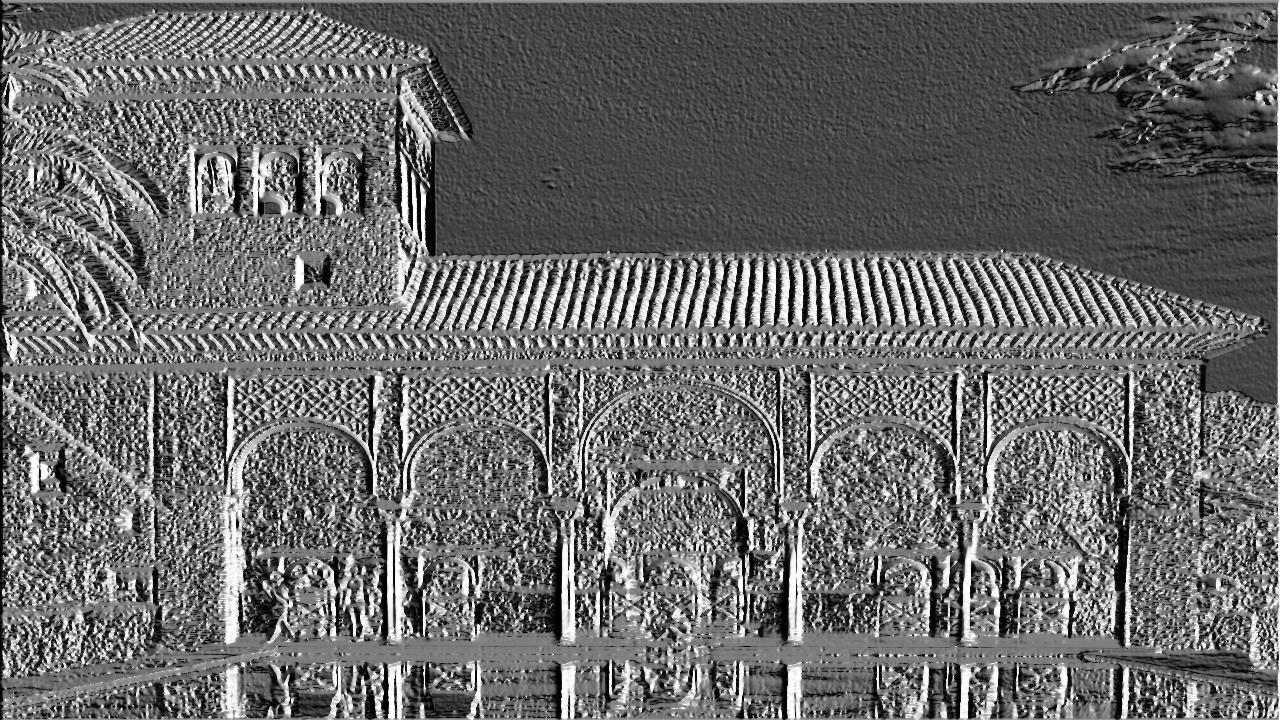
\includegraphics[width= \textwidth]{./figs/mm_dir}
         \caption{absolute value of tangent inverse}
         \label{fig:magtan}
     \end{subfigure}
     \caption{Two alternatives for representing gradient directions}
        \label{fig:magtantan}
\end{figure}
Fig.~\ref{fig:magtantan} shows the difference. It is seen that Fig.~\ref{fig:magtan} has a higher contrast.~\cite{Dalal2005} also uses the same representation and this increases the accuracy up to one percent per dataset.

So the magnitude of gradient can be accompanied by gradient direction in a full-reference manner that we called it gradient similarity~\cite{cheraaqee2019incorporating}. In the next section we use gradient direction in a NR method.
\section{The NR Method}
The proposed NR method is a feature-based method in which, a vector is extracted from the image and a model maps it to a score. The algorithm for extracting the features and the model are explained in the following sub-sections.
\subsection{Extracting Direction-Based Features}
Considering its effect in increasing the accuracy of the FR method, gradient direction sounds to be a good descriptor for quality. Therefore, we were motivated to incorporate it in NR assessment. The purpose here is to code the quality-relevant aspects of an image in a feature vector. Simple histogram of pixel values is not suitable, due to redundancy and a high-dimension.

To shrink the size of feature vector, the values can be quantized. If $v$ is the value of a pixel in the $GD$, then $v\in[0, 180]$. If we want to quantize $v$ to 11 values, the truncated $v$ is defined as:
\begin{equation}
    v_q = \lfloor \frac{v}{18} \rfloor
    \label{eq:qdir}
\end{equation}
and $v_q\in \{0, 1, 2, \ldots, 10\}$. Then the histogram of $GD$ will have 11 bins. Fig.~\ref{fig:hst_dir} shows such histogram for various qualities of two different scenes. The quality decreases from top to bottom.

The features that describe quality, must be independent from image content and correlated with distortions. We see in Fig.~\ref{fig:hst_dir} that quantized directions are independent from the scene, but do not change with the perceived quality. The bins are quite similar for the second and third row and do not distinguish their quality.
\begin{figure}
         \centering
         \includegraphics[width=\textwidth]{./figs/bank_H_D.jpg}
     \caption{Histogram of direction values after quantization}
        \label{fig:hst_dir}
\end{figure}

by weighting the bins with gradient magnitude, we can encode their relation in the histogram. In Fig.~\ref{fig:hst_w_dir} we see that this is effective for sensitivity to quality. Such weighting considers micro and macro structures which have their own sensing mechanisms in HVS~\cite{Griffin2007}.
\begin{figure}
         \centering
         \includegraphics[width=\textwidth]{./figs/bank_MWH_D.jpg}
     \caption{Weighted histogram of direction values}
        \label{fig:hst_w_dir}
\end{figure}

In a local region, the direction of gradient vectors are highly coherent and they are usually computed within $8\times 8$ windows~\cite{Dalal2005}. So in order to extract the local structural deviation, we compute the gradient magnitude of $GD$ with~\ref{eq:gm_gd} and name it $GM_{GD}$. $GM_{GD}$ increases with this deviation (Fig~\ref{fig:mg_dir}). Also, this derivation whitens the information in $GD$.
\begin{equation}
    GM_{GD}(x, y) = \sqrt{\left(\frac{\partial}{\partial x}GD(x, y) \right)^2+\left(\frac{\partial}{\partial y}GD(x, y) \right)^2}
    \label{eq:gm_gd}
\end{equation}

\begin{figure}
     \centering
     \begin{subfigure}[b]{0.24\textwidth}
         \centering
         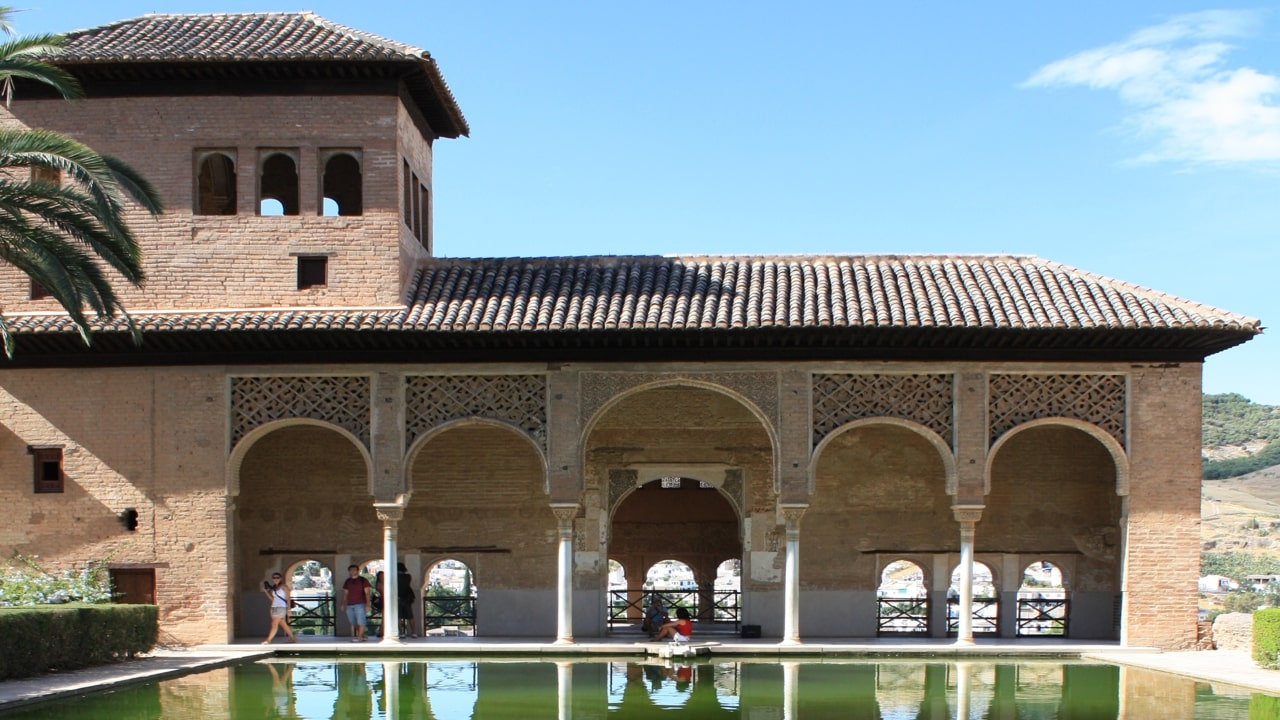
\includegraphics[width=\textwidth]{./figs/org009.jpg}
         \caption{original image\\.}
         \label{}
     \end{subfigure}
     \hfill
     \begin{subfigure}[b]{0.24\textwidth}
         \centering
         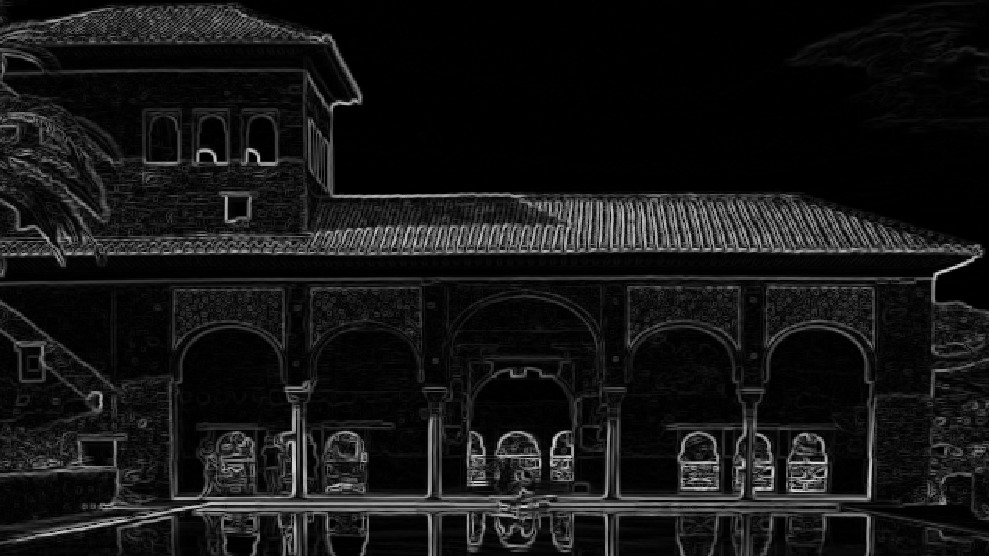
\includegraphics[width= \textwidth]{./figs/mg_map_ref}
         \caption{gradient magnitude of (a)}
         \label{}
     \end{subfigure}
     \hfill
     \begin{subfigure}[b]{0.24\textwidth}
         \centering
         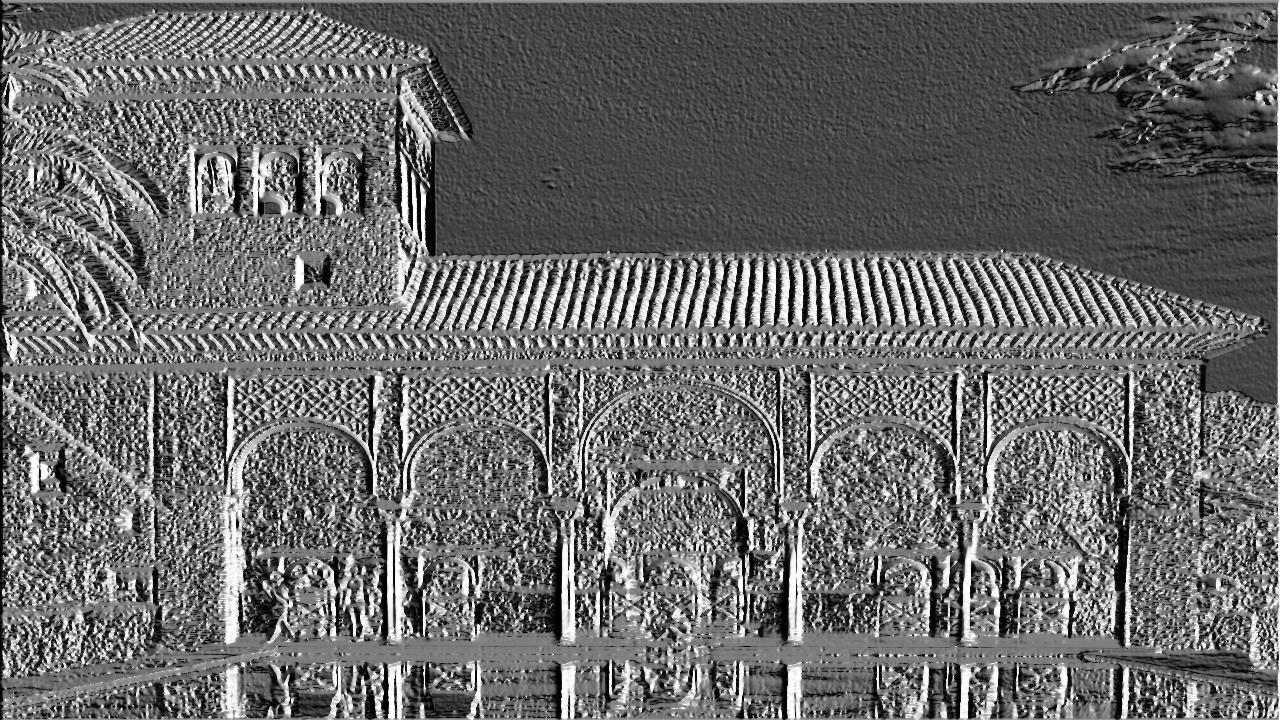
\includegraphics[width= \textwidth]{./figs/mm_dir}
         \caption{gradient magnitude of (d)}
         \label{}
     \end{subfigure}
     \hfill
     \begin{subfigure}[b]{0.24\textwidth}
         \centering
         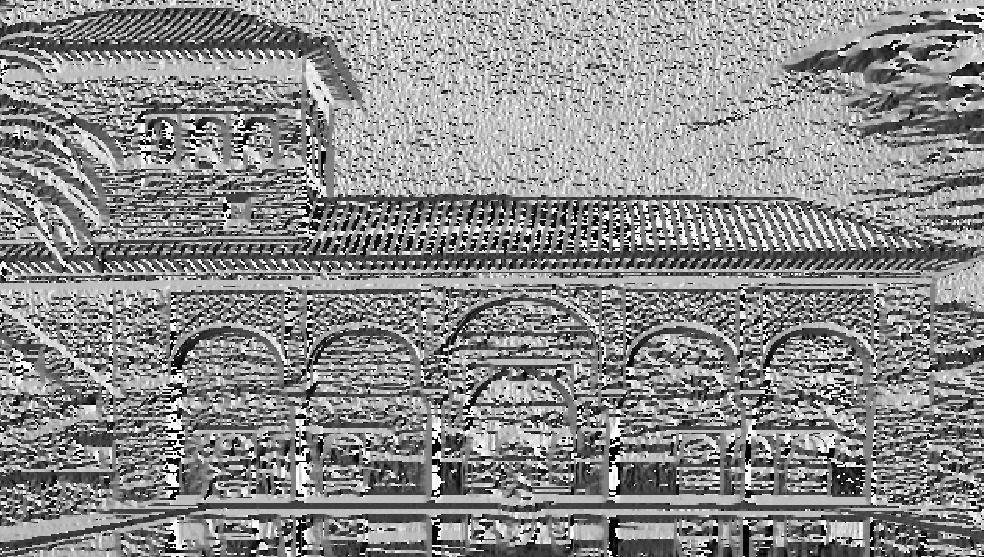
\includegraphics[width= \textwidth]{./figs/dir_ref}
         \caption{gradient direction of (a)}
         \label{}
     \end{subfigure}
     \caption{Gradient magnitude and direction for (a) in (b) and (d), respectively. Derivative of gradient direction in (c)}
        \label{fig:mg_dir}
\end{figure}

To reduce the dimensions and extract NSS, we employed LBPs instead of quantizing the maps. LBP is expressive and describes textures. It was pointed out in IMLBP~\cite{Yue2018} that the sampling rate of HVS drops when getting away from the gazing point~\cite{Pelli2008}. Hence, they changed the operation of LBP to model this phenomenon.

In $LBP_{P, R}^{riu2}$, the difference of the center pixel, $n_c$ and the neighbors, $n_i$ is computed, where $i=1,2, \ldots, P$ (Fig.~\ref{fig:two_lbps_normal}). To simulate the HVS mechanism, a neighborhood of $n_i$ is considered with size $(R-1)\times(R-1)$ (Fig.~\ref{fig:two_lbps_gu}~\cite{Yue2018}). The median value of this neighborhood is addressed as $M_{n_i}$. Then we subtract $n_c$ from $M_{n_i}$s and name the new operator `$MLBP^{riu2}_{P, R}$'.
\begin{figure}
     \centering
     \begin{subfigure}[b]{0.25\textwidth}
         \centering
         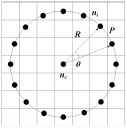
\includegraphics[width= \textwidth]{./figs/lbp_nr}
         \caption{}
         \label{fig:two_lbps_normal}
     \end{subfigure}
     \hfill
     \begin{subfigure}[b]{0.3\textwidth}
         \centering
         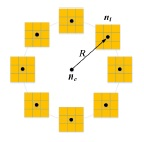
\includegraphics[width= \textwidth]{./figs/lbp_gu}
         \caption{}
         \label{fig:two_lbps_gu}
     \end{subfigure}
     \caption{Difference of $LBP^{riu2}_{P, R}$ and $MLBP^{riu2}_{P, R}$. (a) in $LBP^{riu2}_{P, R}$ the difference of $n_c$ and $P$ $n_i$s is computed, where $n_i$s are located in a neighborhood of radius $R$ and arcs with angles~$\theta=\frac{360}{P}$ (b) a neighborhood of size $3\times 3$ is shown around each $n_i$. The `median' of each neighborhood is considered for subtracting from $n_c$}
        \label{fig:two_lbps}
\end{figure}

$MLBP^{riu2}_{8, 1}$ can obtain one of 10 possible values in $\{0, 1, 2, \ldots, 9\}$. The maps of gradient direction will be described by this operator.

To extract the feature vector of a test image, it is firstly decomposed to $GM$, $GD$, and $GM_{GD}$ maps. The computation of pixels of these maps is formulated in~\ref{eq:gm},~\ref{eq:gd}, and~\ref{eq:gm_gd}. Then, $LBP^{riu2}_{8, 1}$ is computed for $GM$, and $MLBP^{riu2}_{8, 1}$ is computed for $GD$ and $GM_{GD}$. The histograms of the three maps are weighted by $GM$. The final feature vector is the concatenation of these histograms. The same scenes in Fig.~\ref{fig:hst_dir} are described with these features in Fig.~\ref{fig:hst_feat}, where we see the bars fluctuate according to the variation of quality.
\begin{figure}
         \centering
         \includegraphics[width=\textwidth]{./figs/bank_lin_man_cher.jpg}
     \caption{Proposed features for different qualities of two scenes}
        \label{fig:hst_feat}
\end{figure}

For modeling the global precedence principle~\cite{Hughes1996}, feature extraction takes place in multiple scales. Each histogram has 10 bins, so with computing 3 histograms, we end up with a 30-element vector. We compute the vector for 3 scales, so the final feature vector will be of dimension $1\times 90$.
\subsection{Computing the Quality Score}
The workflow of feature-based methods is described in Fig.~\ref{fig:svr_train} and~\ref{fig:svr_test}. If $\Vec{f}_{1\times 90}$ is the extracted feature vector, a model regresses the final score using the features. This model can be a simple arithmetic relation, a neural network, or a SVR.

Although, the method's performance is mainly determined by the expressiveness of the features, for multiple distortions, the model turns out to be very effective~\cite{Dai2018, Yue2018, Zhou2019}. Here we use a SVR~\cite{smola2004tutorial}.

SVR model is a function, $F$ that combines the elements of $\Vec{f}$ to the quality score as in~\ref{eq:svr}, where $\Vec{\omega}$ and $\Vec{b}$ are the weights. If $(\Vec{f}_i, y_i)$ is a sample from a dataset and $y_i$ is the human label, for $i\in \{1, \ldots, N\}$, then the SVR computes the optimum values for $\Vec{\omega}$ and $\Vec{b}$~\cite{chang2011libsvm}.
\begin{equation}
    F(\Vec{f}) = \Vec{\omega}.\Vec{f}^T+\Vec{b}
    \label{eq:svr}
\end{equation}
\section{Summary}
In this chapter we used the direction of gradient vectors to describe the quality of images in a FR and a NR scenario. In the next chapter we evaluate the speed and accuracy of the proposed methods.